Basicly, the recursive implementation calculates the odd and even part of the FFT like a binary tree. All left nodes in the recursive call tree calculate the even part and the odd part is calculated by the right nodes. Parent nodes need the children's result for their own calculations. That's why our arrays get swapped. 
The resulting memory access pattern is as follows:
\begin{center}
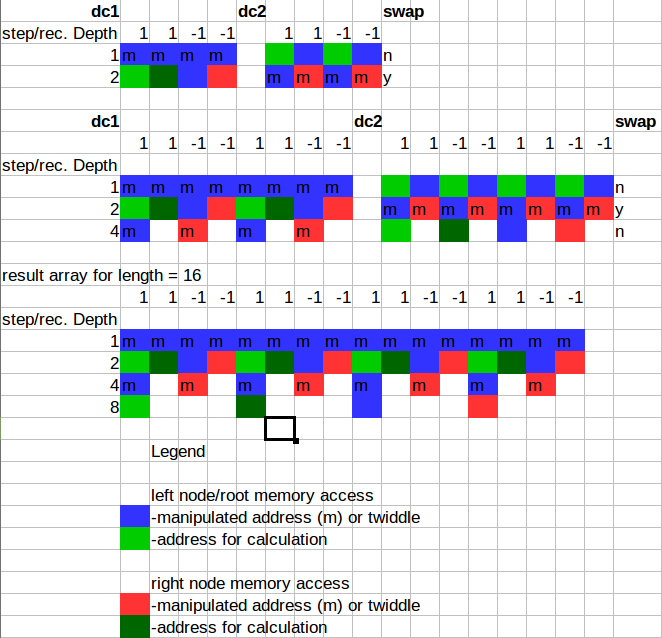
\includegraphics[width=\textwidth]{memacc.png}
\end{center}
The 1's and -1's are just from an example rectangle signal. The picture shows the full memory access for arrays of length 4 and 8. This information is all that you need since you can easily iterative expand the access picture in two steps:
\begin{enumerate}
\item duplicate the memory pattern horizontally
\item copy the last line of the other array, add double the "whitespaces" + 1 after the single accesses and add it as last line of the new access pattern. 
\end{enumerate}
As example we also included the result array for length = 16.
